
\section{Basic Models}
I want to create some basic models in this section to  help me visualize the problem; it can also test my conjuncture of the continuous approximations.

Firstly, I wish to find an optimal starting condition --- this leads to the precalculation of the vertical motion. Secondly, I will model the motion of the remaining two axis of motion. Lastly, I will fit various acceleration models using my experience, some calculus, and even polar coordinates.

% straight line
\subsection{Key idea and boundary conditions}
The key idea that is repeated throughout this analysis is the extent that maximizing the player's velocity or acceleration will maximize the displacement. I hypothesized this from the positional differential equations in Eq. \ref{eq:1de2}, where under the assumption of constant velocity the final displacement will be proportional to that constant:
\begin{align*}
    \tp'(t) &= \tv(t)\\
    \tp(t) &= \int \tv(t) \, dt\\
    &= t\tv(t) + \tp(0) = t\tv(t) + \tzero,\\
    \tp &\propto \tv(t).
\end{align*}

Using this idea, I devised an optimal initial velocity for the player --- this also known as the boundary condition of the problem. For we are maximizing the jump displacement, and higher velocity equates to higher displacement, it is reasonable to set the initial velocity/speed as high as possible. So
\[
    \tmag{\tv} = 250,
\]
where $250$ is fastest ground running speed.


\begin{figure}[H]
    \centering
    \begin{minipage}{.5\textwidth}
        \centering
        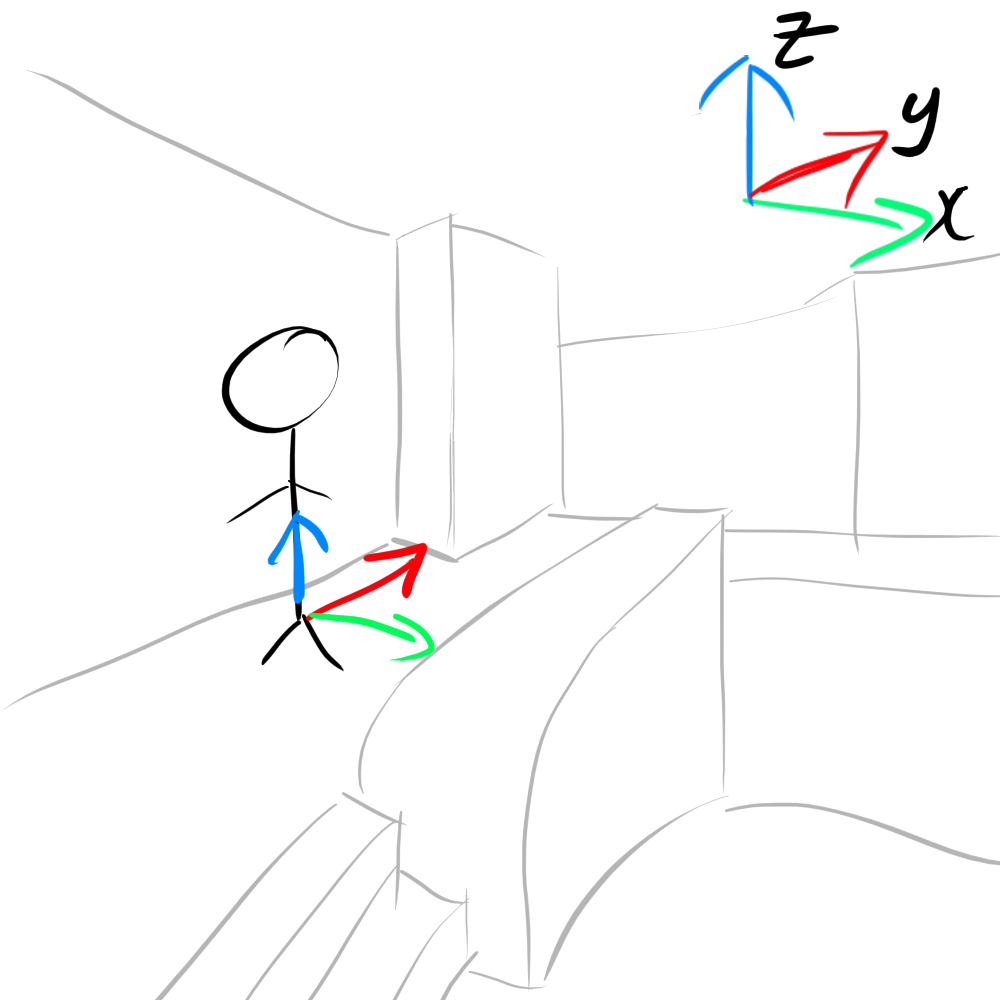
\includegraphics[width=0.9\linewidth]{assets/1coordinates.png}
        \caption{The coordinate system}
        \label{fig:1coordinates}
    \end{minipage}%
    \begin{minipage}{.5\textwidth}
        \centering
        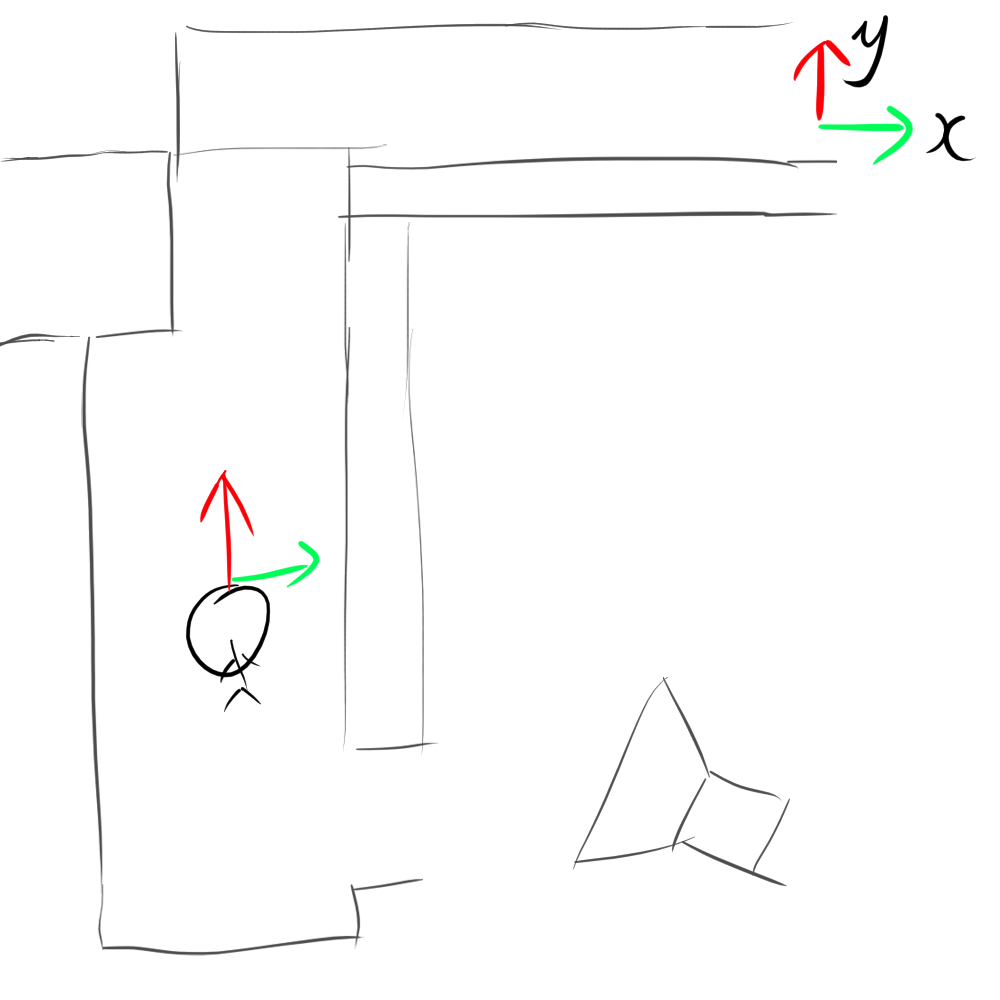
\includegraphics[width=0.9\linewidth]{assets/2coordinate_topdown.png}
        \caption{The top down view}
        \label{fig:2coordinates_topdown}
    \end{minipage}
\end{figure}


Furthermore, the problem is top-down rotationally invariant. Let the z-axis denote the vertical height of the player, and the x,y-axis to be the plane displacement from a top down view (see figure \ref{fig:1coordinates}, figure \ref{fig:2coordinates_topdown}).

In considering only the x,y-axis, I realized that an optimal strategy does not depend on the angle of the initial velocity vector within the plane, for it is always possible to rotate the initial velocity so that we travel in a desired direction of displacement (see the blue vector and purple curve in figure \ref{fig:2turning}). This meant that the optimal initial velocity is not restricted to a certain direction, but for the sake of consistency between models, I shall use the initial velocity pointing in the y-axis:
\[
    \tv(0) = \tang{0, 250, 0}.
\]

\begin{wrapfigure}{r}{0.40\textwidth}
    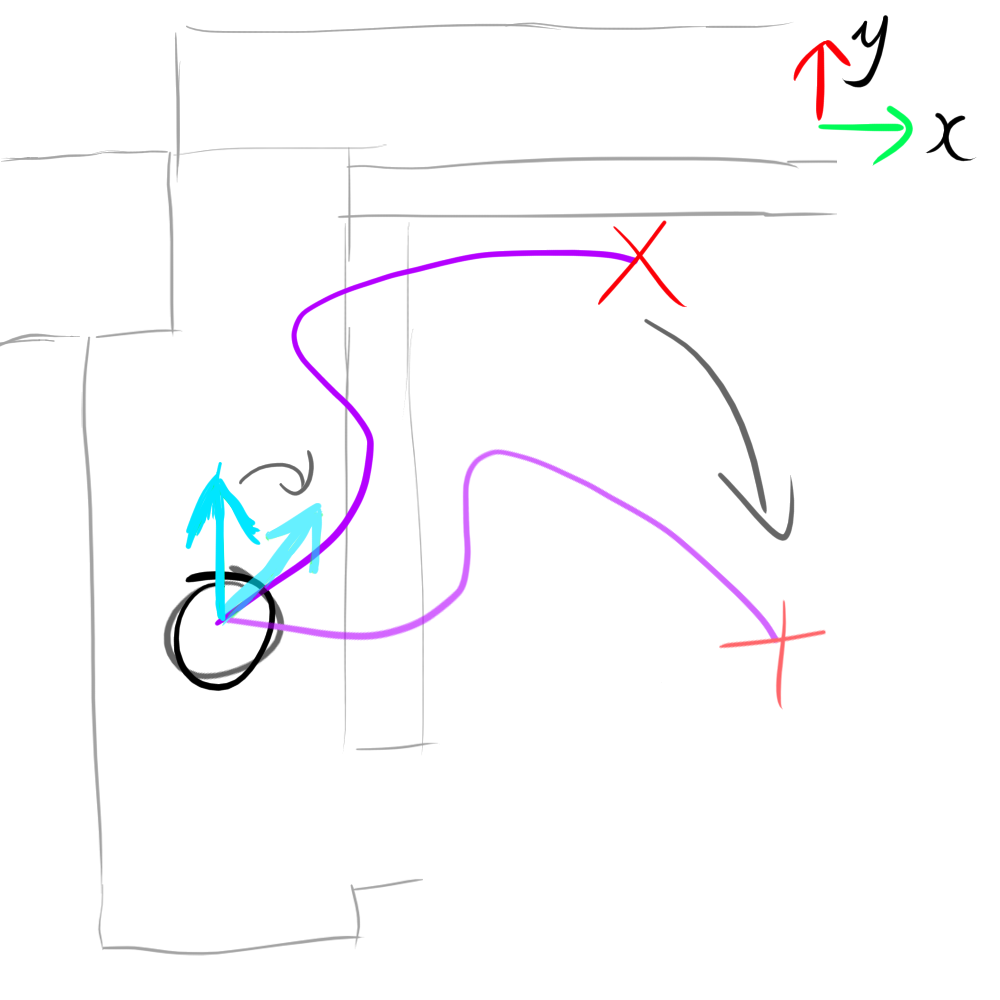
\includegraphics[width=0.37\textwidth,right]{assets/2turning.png}
    \caption{Rotational Invariant (the player wishes to go rightwards)}
    \label{fig:2turning}
\end{wrapfigure}


Additionally, let the initial position of the player to be zero for ease of calculations:
\[
    \tp(0) = \tang{0, 0, 0}
\]


The z-axis initial velocity must be experimentally determined. This is because the player cannot supply any initial vertical velocity as it is moving on a x,y-plane prior to the jump, so the only vertical velocity comes from the action of the jump. In fact, we will soon see that the z-axis can be precomputed to reduce the dimensionality of the problem.

\subsection{Straight line model}

With the key idea and boundary conditions in mind, I attempted a straight line strategy. This model has the player accelerate and move in a straight line, as mathematics has taught me that the shortest displacement between two points comes from a line, reducing the unnecessary displacements if all I was optimizing is the total displacement. To achieve this, the player would need to accelerate along its initial velocity of the y-axis. Mathematically, this is equivalent to setting the directional vector to
\[
    \td(t) = \tang{0, 1}
\]
at all times. Realistically, this will be equivalent to pressing down the move forward button and not moving the mouse that turns the player.
% do model!!
\begin{figure}[H]
    \centering
    \begin{minipage}{.5\textwidth}
        \centering
        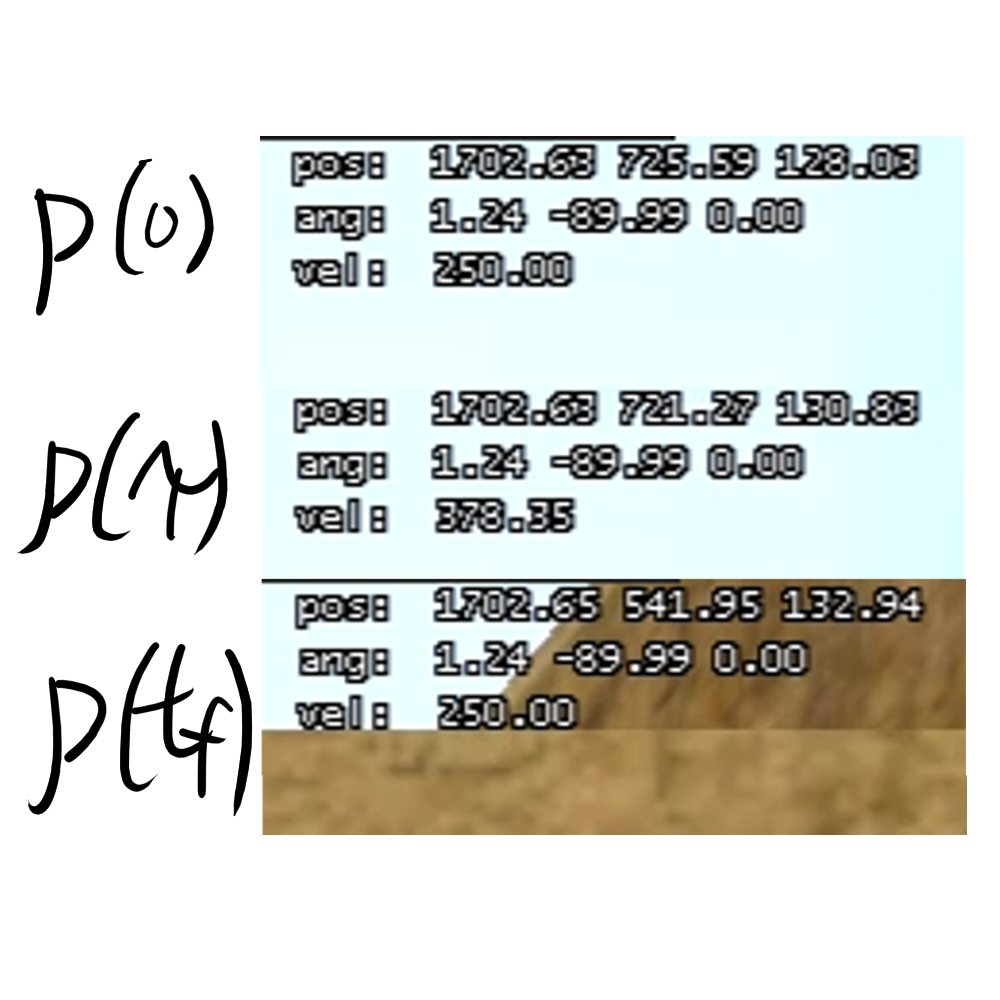
\includegraphics[width=0.9\linewidth]{assets/2straightjumping.png}
        \caption{Straight Jumping}
        \label{fig:2straightjumping}
    \end{minipage}%
    \begin{minipage}{.5\textwidth}
        \centering
        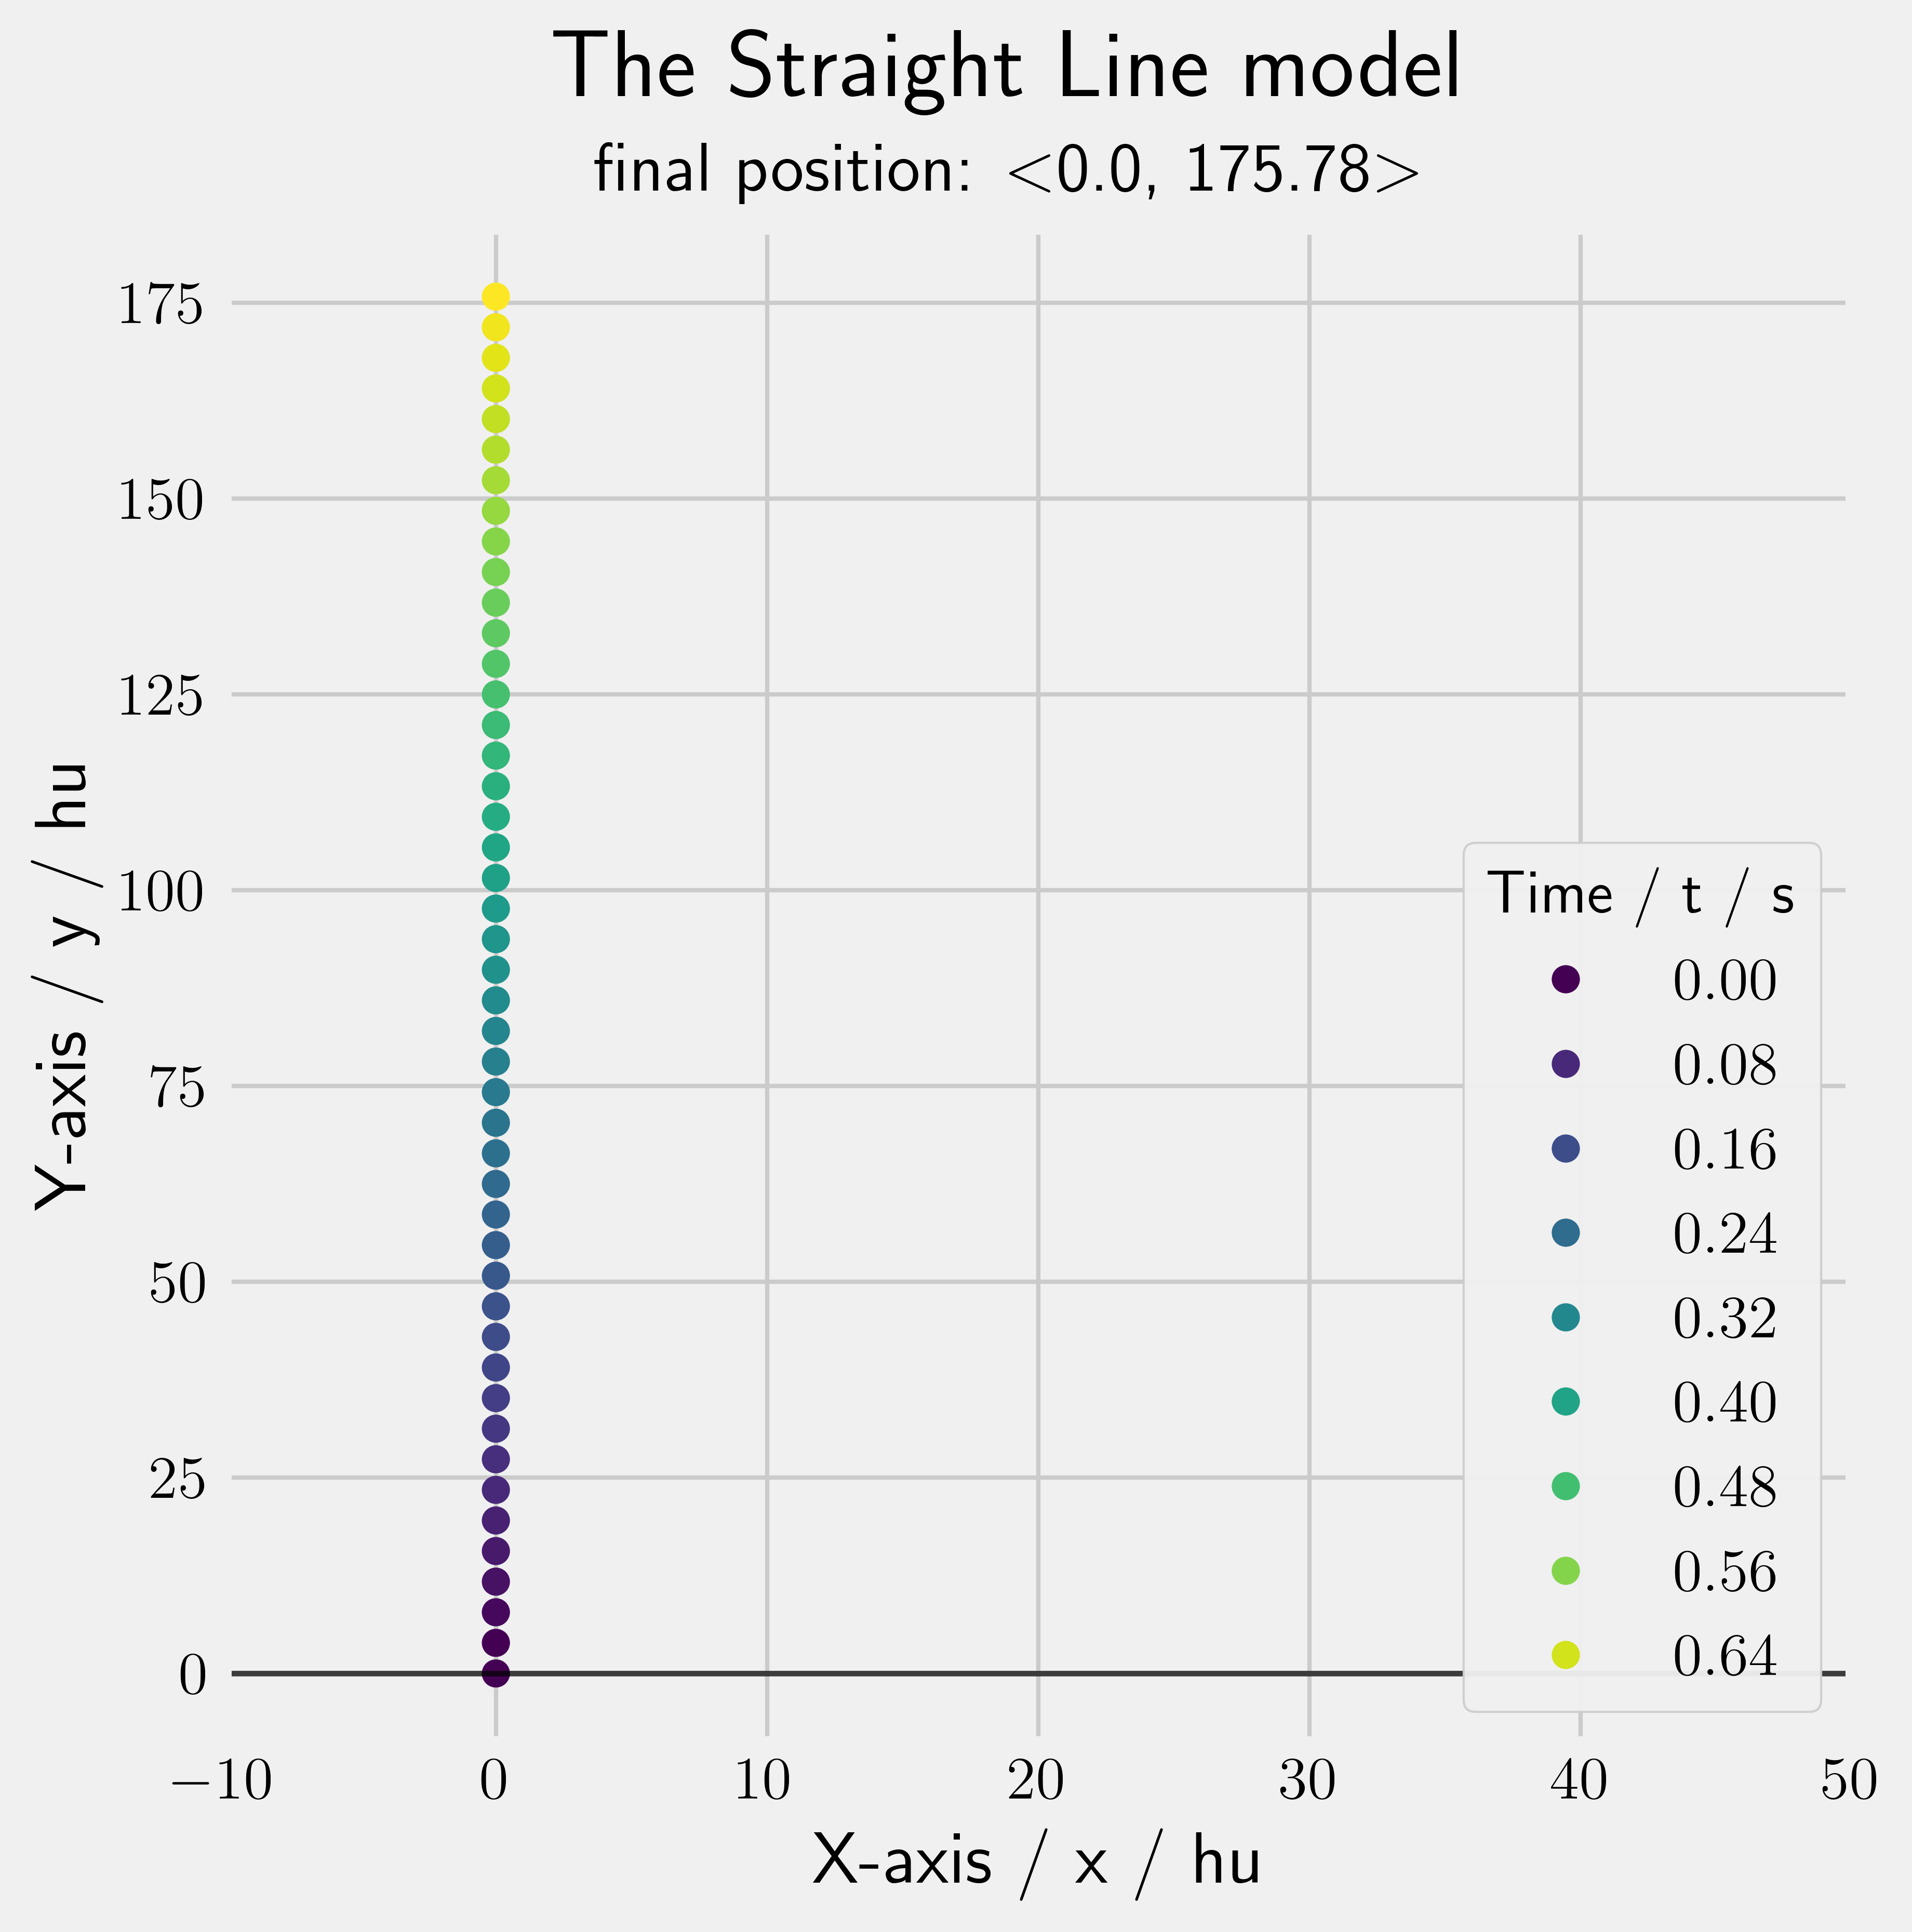
\includegraphics[width=0.9\linewidth]{assets/straight_constraint.png}
        \caption{Simulated Player Movement}
        \label{fig:straight_constraint}
    \end{minipage}
\end{figure}

To test this model, I recorded myself jumping and performing the actions described above. Ideally the x,z-axis shouldn't be changed as I am moving along the y-axis only. Figure \ref{fig:straight_constraint} shows the estimation of the player's path using software; Figure \ref{fig:2straightjumping} shows the coordinates of the player at the start of the jump $\tp(0)$, the first frame of the jump $\tp(\tau)$, and the end of the jump $\tp(t_f)$, where the symbol $t_f$ denotes the duration of the jump:
\begin{align}
 \tp(0) &= \tang{1702.63, 725.59, 128.03}, \quad \tmag{\tv(0)} = 250.00 \label{eq:2emp0}\\
 \tp(\tau) &= \tang{1702.63, 721.27, 130.83}, \quad \tmag{\tv(\tau)} = 378.35 \label{eq:2emp1}\\
 \tp(t_f) &= \tang{1702.65,541.95, 132.94}, \quad \tmag{\tv(t_f)} = 250.00 \label{eq:2emp2}.
\end{align}

\subsubsection{Analysis}
With the simple empirical data in Eq. \ref{eq:2emp0}, Eq. \ref{eq:2emp1}, and Eq. \ref{eq:2emp2}, not only can I analyze the straight line model, but it also allows me to model the vertical motion. However, I've noticed that the x,z-axis have changed after the jump. The x change is likely the result of some uncertainty in me pointing the initial velocity directly in the y-axis, but due to the rotational invariant discussed before, this is a non detrimental problem; but the z-axis is different and is likely to be the result of some ``bounciness'' of the player as lands from the jump --- this doesn't matter in the optimizing of displacement. Thus, I chose to ignore the z-axis change during calculations.

The total displacement of this jump par our definition is the expression $d = \tmag{\tp(t_f) - \tp(0)}$, which is
\begin{align*}
    d &= \sqrt{(\tp_x(t_f) - \tp_x(0))^2 + (\tp_y(t_f) - \tp_y(0))^2 + (\tp_z(t_f) - \tp_z(0))^2}\\
    &= \sqrt{(1702.65-1702.63)^2 + (541.95-725.59)^2 + (0)^2}\\
    &\approx 183.64.
\end{align*}

Firstly notice the sudden change in the velocity of the player at in first frame, time $\tau$. From this I deduced that the act of jumping is achieved by an impulse --- a sudden change in velocity --- upon the z-axis. With the assumption that no such impulses occurs in the x,y-axis, and that the x,y-plane acceleration in the first frame is negligible, we can find the size of impulse at the start of the jump using the Pythagorean Theorem (figure \ref{fig:2verticalimpulse}).



\begin{align*}
    \tmag{\tv}^2 &= \tv_y^2 + \tv_z^2\\
    \tv_z &= \sqrt{\tmag{\tv}^2 - \tv_y^2}\\
    &= \sqrt{378.35^2 -250^2}\\
    &= 284.00.
\end{align*}

\begin{wrapfigure}{r}{0.40\textwidth}
    \centering
    %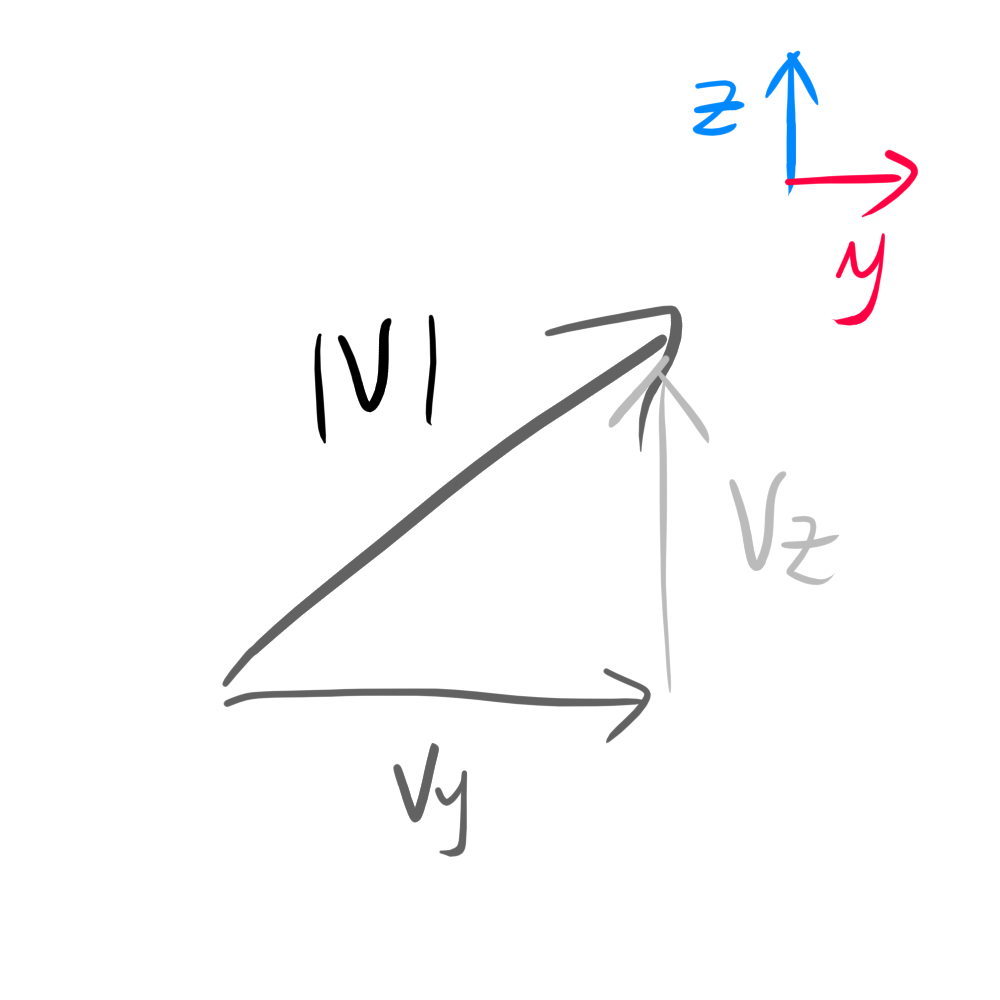
\includegraphics[width=0.37\textwidth,right]{assets/2verticalimpulse.png}
    \sized[0.4]{
        \tikzset{every picture/.style={line width=0.75pt}} %set default line width to 0.75pt        

        \begin{tikzpicture}[x=0.75pt,y=0.75pt,yscale=-1,xscale=1]
        %uncomment if require: \path (0,236); %set diagram left start at 0, and has height of 236

        %Shape: Axis 2D [id:dp8024732250876303] 
        \draw [color={rgb, 255:red, 0; green, 0; blue, 0 }  ,draw opacity=1 ] (418.43,41.53) -- (450,41.53)(421.59,10) -- (421.59,45.04) (443,36.53) -- (450,41.53) -- (443,46.53) (416.59,17) -- (421.59,10) -- (426.59,17)  ;
        %Straight Lines [id:da935697118906834] 
        \draw    (290,150) -- (377.76,71.99) ;
        \draw [shift={(380,70)}, rotate = 138.37] [fill={rgb, 255:red, 0; green, 0; blue, 0 }  ][line width=0.08]  [draw opacity=0] (10.72,-5.15) -- (0,0) -- (10.72,5.15) -- (7.12,0) -- cycle    ;
        %Straight Lines [id:da37870943266053725] 
        \draw    (290,150) -- (377,150) ;
        \draw [shift={(380,150)}, rotate = 180] [fill={rgb, 255:red, 0; green, 0; blue, 0 }  ][line width=0.08]  [draw opacity=0] (10.72,-5.15) -- (0,0) -- (10.72,5.15) -- (7.12,0) -- cycle    ;
        %Straight Lines [id:da23229694740869355] 
        \draw [color={rgb, 255:red, 74; green, 144; blue, 226 }  ,draw opacity=1 ]   (380,150) -- (380,73) ;
        \draw [shift={(380,70)}, rotate = 90] [fill={rgb, 255:red, 74; green, 144; blue, 226 }  ,fill opacity=1 ][line width=0.08]  [draw opacity=0] (10.72,-5.15) -- (0,0) -- (10.72,5.15) -- (7.12,0) -- cycle    ;

        % Text Node
        \draw (429,42) node [anchor=north west][inner sep=0.75pt]  [xscale=1.25,yscale=1.25] [align=left] {{\fontfamily{pcr}\selectfont y}};
        % Text Node
        \draw (405,21) node [anchor=north west][inner sep=0.75pt]  [xscale=1.25,yscale=1.25] [align=left] {{\fontfamily{pcr}\selectfont z}};
        % Text Node
        \draw (321,160) node [anchor=north west][inner sep=0.75pt]  [color={rgb, 255:red, 80; green, 227; blue, 194 }  ,opacity=1 ,xscale=1.25,yscale=1.25] [align=left] {$\displaystyle \textcolor[rgb]{0,0,0}{v_{y}}$};
        % Text Node
        \draw (311,82) node [anchor=north west][inner sep=0.75pt]  [color={rgb, 255:red, 80; green, 227; blue, 194 }  ,opacity=1 ,xscale=1.25,yscale=1.25] [align=left] {$\displaystyle \textcolor[rgb]{0,0,0}{v}$};
        % Text Node
        \draw (392,102) node [anchor=north west][inner sep=0.75pt]  [color={rgb, 255:red, 80; green, 227; blue, 194 }  ,opacity=1 ,xscale=1.25,yscale=1.25] [align=left] {$\displaystyle \textcolor[rgb]{0.29,0.56,0.89}{v_{z}}$};


        \end{tikzpicture}
    }
    \caption{\vspace{8ex} Jumping impulses}
    \label{fig:2verticalimpulse}
\end{wrapfigure}

With approximations to continuous time, we can set the player's initial vertical velocity to this number such that
\[
    \tv_{z}(0) = 284.
\]


Secondly, by measuring the duration of the jump --- which I've done by counting the number of video frames of a sixty hertz video, or $44 \times \frac{1}{60} \approx 0.7333 \si{s}$ --- I was able to derive the average speed $\tmag{\tv_{a}}$ of the player:
\[
    \tv_{a} = \frac{183.71}{0.7333} \approx 250.42.
\]

Isn't that surprising? Turns out that there is almost zero net acceleration in the straight line model. The average velocity does not differ from its initial value, meaning that the acceleration as a function of time $t$ and wishing direction $\td(t)$ is zero at least in the x,y-axis:
\[
    \ta(t, \td) = \tang{0, 0, ?}.
\]

I suspect a speed limit is in play here. This is bad in the optimization of jump displacement as it restricts the player's velocity, which by the key idea, is likely to limit the displacement too. But it cannot be limiting the magnitude of velocity directly as I've subconsciously achieved higher velocities while playing. My research in the engine source code \parencite{valvesoftware} and a simplified article about the mechanics in a similar game called ``Half Life'' \parencite{jwchong} was targeting exactly this mechanic of velocity limiting. In short, the player's velocity $\tv$ is limited by its projection onto the directional vector $\td$.

\subsubsection{Speed limit}
\begin{wrapfigure}{r}{0.40\textwidth}
    %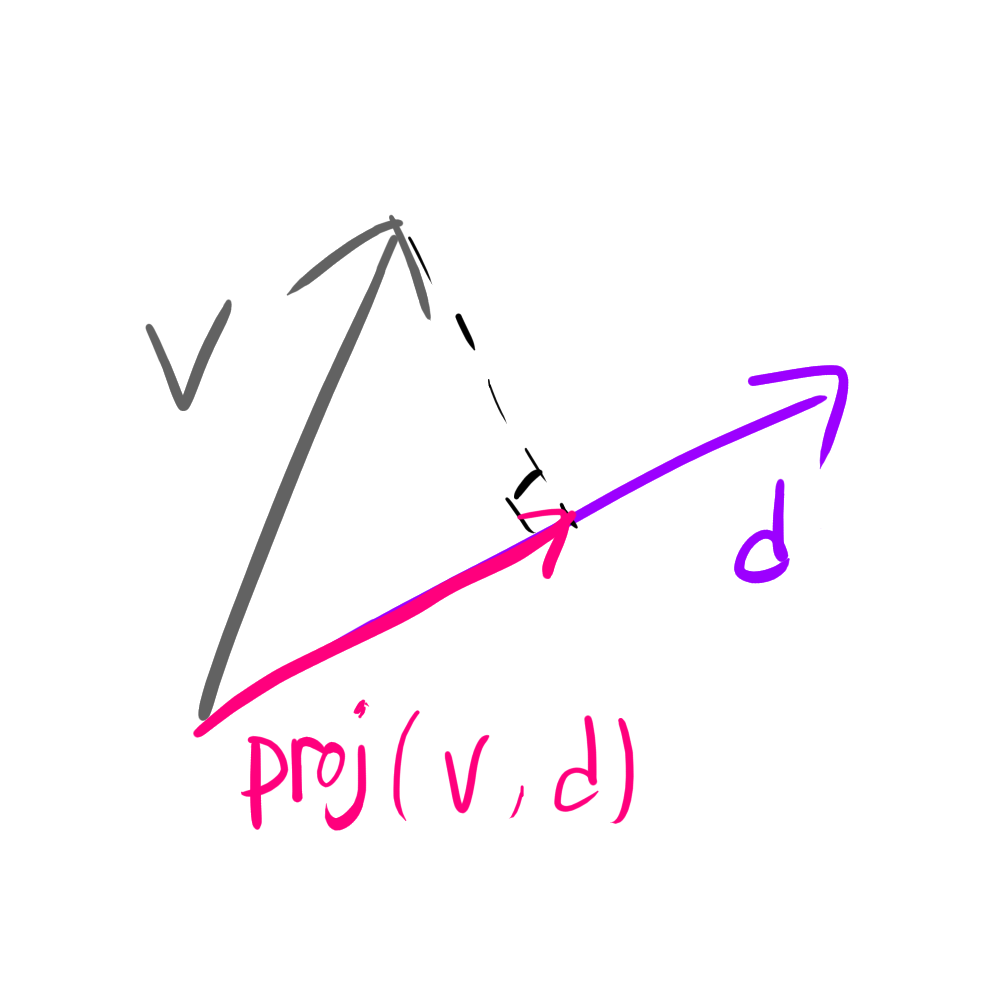
\includegraphics[width=0.37\textwidth,right]{assets/2proj.png}
    \sized[0.4]{
        

\tikzset{every picture/.style={line width=0.75pt}} %set default line width to 0.75pt        

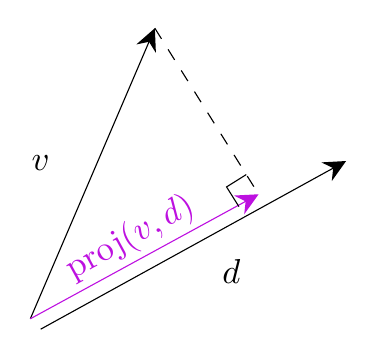
\begin{tikzpicture}[x=0.75pt,y=0.75pt,yscale=-1,xscale=1]
%uncomment if require: \path (0,201); %set diagram left start at 0, and has height of 201

%Straight Lines [id:da88922271648241] 
\draw    (282,170) -- (340.82,32.76) ;
\draw [shift={(342,30)}, rotate = 113.2] [fill={rgb, 255:red, 0; green, 0; blue, 0 }  ][line width=0.08]  [draw opacity=0] (10.72,-5.15) -- (0,0) -- (10.72,5.15) -- (7.12,0) -- cycle    ;
%Straight Lines [id:da11348579225934163] 
\draw [color={rgb, 255:red, 189; green, 16; blue, 224 }  ,draw opacity=1 ]   (282,170) -- (389.37,111.44) ;
\draw [shift={(392,110)}, rotate = 151.39] [fill={rgb, 255:red, 189; green, 16; blue, 224 }  ,fill opacity=1 ][line width=0.08]  [draw opacity=0] (10.72,-5.15) -- (0,0) -- (10.72,5.15) -- (7.12,0) -- cycle    ;
%Straight Lines [id:da5945932118539943] 
\draw  [dash pattern={on 4.5pt off 4.5pt}]  (342,30) -- (392,110) ;
%Shape: Right Angle [id:dp9723060706204649] 
\draw   (382.51,115.95) -- (376.55,106.46) -- (386.05,100.51) ;
%Straight Lines [id:da7502223575804331] 
\draw    (287,175) -- (431.52,95.43) ;
\draw [shift={(434.15,93.98)}, rotate = 151.16] [fill={rgb, 255:red, 0; green, 0; blue, 0 }  ][line width=0.08]  [draw opacity=0] (10.72,-5.15) -- (0,0) -- (10.72,5.15) -- (7.12,0) -- cycle    ;

% Text Node
\draw (294.24,139.42) node [anchor=north west][inner sep=0.75pt]  [color={rgb, 255:red, 189; green, 16; blue, 224 }  ,opacity=1 ,rotate=-331.37,xscale=1.25,yscale=1.25] [align=left] {proj$\displaystyle ( v,d)$};
% Text Node
\draw (281,90) node [anchor=north west][inner sep=0.75pt]  [xscale=1.25,yscale=1.25] [align=left] {$\displaystyle v$};
% Text Node
\draw (373,140) node [anchor=north west][inner sep=0.75pt]  [xscale=1.25,yscale=1.25] [align=left] {$\displaystyle d$};


\end{tikzpicture}

    }
    \caption{\vspace{8ex} Projection limiting}
    \label{fig:2proj}
\end{wrapfigure}

A vector's projection onto another is a way to say how much of the vector is pointing in the direction of another, in the form of a number. Denoted by $\text{proj}(\tv, \td)$, the projection of the player's velocity vector onto its direction vector is the side of the triangle formed by a perpendicular line from $\tv$ to $\td$ (figure \ref{fig:2proj}). This can be defined using a dot product:
\[
    \text{proj}(\tv, \td) = \frac{\tv \cdot \td}{\tmag{\td}}.
\]

Also, because the z-component of $\td$ is always zero, the projection is simply the 2D vector dot product between $\tv$ and $\td$.
\begin{align*}
    \text{proj}(\tv, \td) &= \tv \cdot \td\\
    &= \tv_x \td_x + \tv_y \td_y + \tv_z \td_z\\
    &= \tv_x \td_x + \tv_y \td_y.
\end{align*}

Crucially, the limits the player's velocity through this projection vector against the value $L$, set to $250$. If the projection exceeds $L$, acceleration will be zero; else, acceleration is a constant in the direction of $\td$ equal to $LA\tau$ in the discrete sense, and $LA$ in the continuous approximation --- with $A$ being a multiplier equal to $10$. The player's 2D acceleration function can therefore be defined piecewisely as:
\begin{figure}[H]
    \centering
    \[
        \ta(t) = \begin{cases}
            LA \td & \text{proj}(\tv, \td) < L\\
            0 & \text{otherwise}
        \end{cases}
    \]
        \caption{Player 2D acceleration function}
    \label{eq:playeracceleration}

\end{figure}

In the case of maximizing displacement, we would want the first condition of equation \ref{eq:playeracceleration} to be true for as long as possible. Yet in the context of my straight line model, it is simple to see that the first condition is never true, for
\begin{align*}
    \text{proj}(\tv, \td) &= \tv_x \td_x + \tv_y \td_y\\
    &= \tv_x \times 0 + \tv_y \times 1\\
    &= \tv_y,\\
    \text{and because} \quad \tv_{y}(0) &= 250 = L\\
    \text{proj}(\tv, \td) &= L\\
    \text{and} \quad \ta(t) &= 0.
\end{align*}

Therefore, my acceleration model has confirmed my hypothesis that the player is not accelerating in the x,y-axis at all. This makes the model a terrible one for maximizing one's jumping displacement, as low acceleration equates to lower velocity, and in turn decreases displacement per my key idea.

\subsubsection{Continuous modeling approximation}
But before I try some other models, let's first evaluate the accuracy of an continuous approximation using this simplistic model. The game engine's code reveals a universal gravitational acceleration $g$ of value $800$, and I thought of this as an opportunity to test my continuous approximation by comparing my calculated value with the real value.

The objective is to solve the differential equations of motion for the player. For the x,y-axis acceleration of the player is zero, and let $g$ be the signed z-axis acceleration:
\[
    \ta = \tang{0, 0, g},
\]
the velocity as defined in Eq. \ref{eq:1de1} is the integral of acceleration:
\begin{align*}
    \tv &= \int \ta \, dt\\
    &= \tang{0, 0, gt} + \tv(0)\\
    &= \tang{0, 250, gt + 284}.
\end{align*}

Continuing, the player position is the integral of velocity as shown in Eq. \ref{eq:1de2}:
\begin{align*}
    \tp &= \int \tv \, dt\\
    &= \tang{0, 250t, \frac{1}{2}gt^2 + 284t} + \tp(0)\\
    &= \tang{0, 250t, \frac{1}{2}gt^2 + 284t}
\end{align*}
shows that the the y-axis displacement is $250t$. Because the actual displacement is $\approx 183.64$, this means that the jump duration $t_f$ is
\[
    t_f = \frac{183.64}{250} \approx 0.735 \si{s}.
\]
Thus, since the z-axis displacement is zero, the gravitational acceleration $g$ is calculated to be
\begin{align*}
    \tp_{z}(t_f) &= \frac{1}{2}gt_f^2 + 284t_f = 0\\
    g &= - 2 \times \frac{284t_f}{t_f^2}\\
    &= -\frac{568}{t_f}\\
    &\approx -772.79.
\end{align*}

Comparing to the actual value of $g=800$, the strength of $772.79$ is not far off --- the relative error of $\frac{800 - 772.79}{800} = 3.4\%$ is close enough for an approximation. Therefore it is justified that for the rest of the models that I can continuously use the continuous approximations, to which I will.

\subsection{Skilled player's model}
A better strategy would be the player accelerating not directly along their velocity, but rather at an angle to their velocity. Personally I've been told by numerous skilled players that you need to move your mouse slowly to the right --- meaning rotating the vector $\td$ over time --- to get higher speed and distance. Now I can test this theory.

Currently, any strategy is uniquely defined by the player's direction function $\td(t)$ as a real 2-vector. Ideally, this vector should be pointing along the y-axis at $t=0$, and rotate clockwise over time. This reminded me of a unit circle, albeit with the x,y-axis switched, creating
\[
    \td(t) = \tang{\sin(t), \cos(t)}.
\]
One can verify that this definition both denote rotation over time and have a magnitude of $1$. Furthermore, I can encode the rate of rotation by scaling the inner $t$ in the two trig functions by the same factor $w$. Therefore, the player direction function $\td(t)$ as recommended by skilled players is
\[
    \td(t) = \tang{\sin(wt), \cos(wt)}.
\]

My task is to find the best constant $w$ that maximizes displacement. The plan is to solve the x,y-axis differential equation into a function of position $\tp$, then explicitly writing the speed limit as an inequality constraint, and finally selecting the constant $w$ that (hopefully) satisfies the constraint and maximizes the displacement.

\subsubsection{Displacement equation}
The key idea suggests that I should maximize the velocity, and as explained in the previous subsection, this meant that player acceleration $\ta$ is to be maximized by fulfilling the inequality projection in equation \ref{eq:playeracceleration}. Thus by assumption that this inequality is held,
\[
    \ta(t) = LA\td.
\]

Let $k=LA$. Notice that the velocity is the integral of acceleration,
\begin{align*}
    \tv(t) &= \int \ta \, dt\\
    &= \int k \tpar{\sin(wt)}{\cos(wt)} \, dt\\
    &= \frac{k}{w} \tpar{-\cos(wt)}{\sin(wt)} + c_v,\\
    \tv(0) &= \frac{k}{w} \tpar{-\cos(0)}{\sin(0)} + c_v\\
    c_v &= \frac{k}{w} \tpar{1}{0} + \tpar{\tv_x(0)}{\tv_y(0)}.
\end{align*}

And the position is the integral of velocity,
\begin{align*}
    \tp(t) &= \int \tv \, dt\\
    &= \int \frac{k}{w} \tpar{-\cos(wt)}{\sin(wt)} + \frac{k}{w}\tpar{1}{0} + \tpar{\tv_x(0)}{\tv_y(0)} \, dt\\
    &= \frac{-k}{w^2} \tpar{\sin(wt)}{\cos(wt)} + \frac{k}{w}\tpar{t}{0}  + t\tpar{\tv_x(0)}{\tv_y(0)} + c.
\end{align*}

To find the integration constant $c$, consider the x-axis displacement function
\begin{align*}
    \tp_x(t) &= \frac{-k}{w^2} \sin(wt) + t\tv_x(0) + t\tv_x(0) + c_x = 0\\
    c_x &= 0,
\end{align*}
and the y-axis displacement function
\begin{align*}
    \tp_y(t) &= \frac{-k}{w^2} \cos(wt) + t\tv_y(0) + c_y = 0\\
    c_y &= \frac{k}{w^2}.
\end{align*}

Using the Pythagorean Theorem, the magnitude of the player's displacement using this model after a jump at $t=t_f$ is:
\begin{figure}[H]
    \centering
    \begin{align*}
        \tmag{\tp(t_f) - \tp(0)} &= \sqrt{\tp_x(t_f)^2 + \tp_y(t_f)^2}\\
        &= \sqrt{\left(\frac{-k}{w^2}\sin(wt_f) + t_f\frac{k}{w} \right)^2 + \left( \frac{-k}{w^2}\cos(wt_f) + 250t_f + \frac{k}{w^2} \right)^2}
    \end{align*}
    \caption{Skilled Displacement}
    \label{eq:2skilled_displacement}

\end{figure}

\begin{figure}[H]
    \centering
    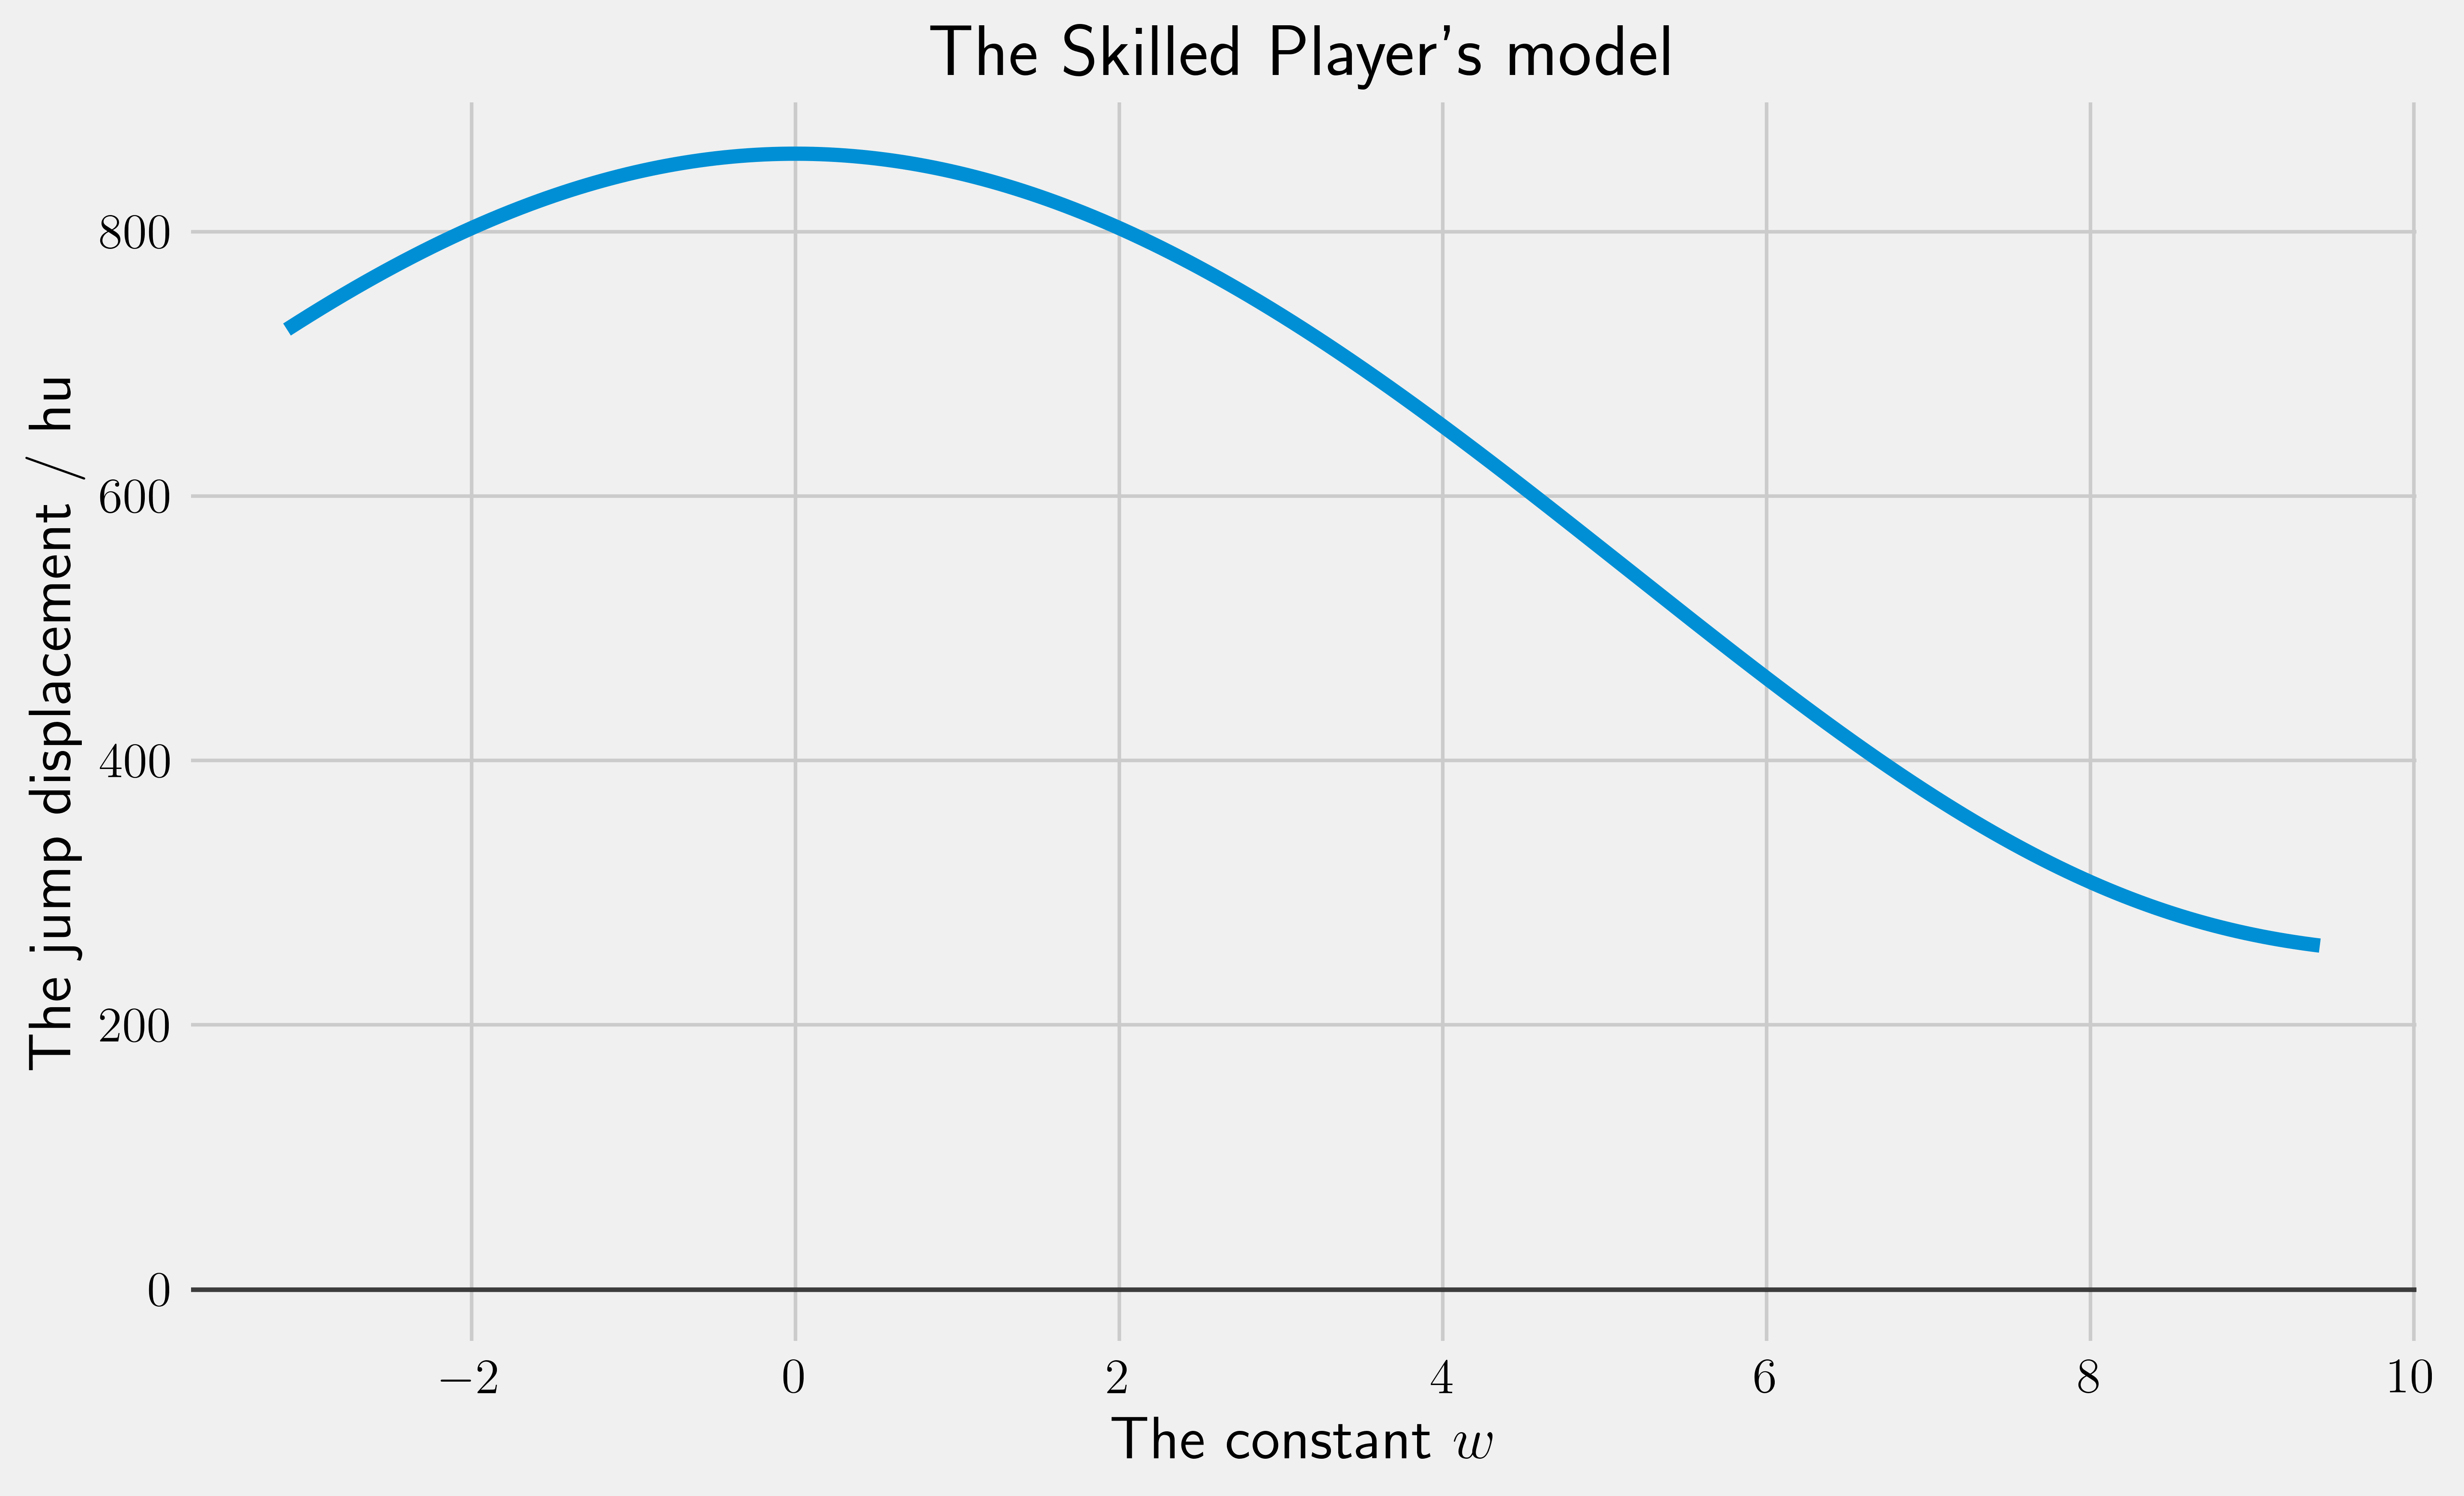
\includegraphics[width=0.85\textwidth]{assets/skilled_displacement.png}
    \caption{}
    \label{fig:skilled_displacement}

\end{figure}
The graph of equation \ref{eq:2skilled_displacement} shown in figure \ref{fig:skilled_displacement} is symmetrical along the y-axis. This is because of yet another symmetry between a left-turning and a right-turning jump. Quantitatively, this ``unlimited'' strategy peeks when $w=0$ when the strategy collapses to my straight line model. As the turning speed $w$ increases, the ideal displacement decreases and levels near $w=10$: I guess that a spinning player does not contribute much to jumping far. Therefore we need to choose the smallest $w$ possible to maximize potential jump displacement.

\subsubsection{Restriction equation}
In addition to finding the ``unlimited'' displacement of the strategy for all constants $w$, we also need check if they satisfy the assumption of unrestricted acceleration at all times. Ideally there should be a value of $w$ that always fits this constraint, but the smallest ``error'' from the ideal is always a backup option.

As shown in figure \ref{eq:playeracceleration}, for maximum acceleration of $\ta(t) = LA\td$, the constraint
\[
    \text{proj}(\tv, \td) < L
\]
must be held for the duration of the jump from $t=0$ to $t=t_f$. Expanding and organizing this inequality yields
\begin{align*}
    L &> \text{proj}(\tv, \td)\\
    &> \tv_x \td_x + \tv_y \td_y\\
    &> \left(-\frac{k}{w} \cos(wt) + \frac{k}{w}\right) \sin(wt) + \left(\frac{k}{w} \sin(wt) + 250\right) \cos(wt),\\
    0 &> \left(-\frac{k}{w} \cos(wt) + \frac{k}{w}\right) \sin(wt) + \left(\frac{k}{w} \sin(wt) + 250\right) \cos(wt) - 250
\end{align*}

To find the value of the constant $w$ that best fulfills this inequality would need a quantitative measure on how well this inequality is held through the jump. Ideally the function should only include the failures of fulfilling the inequality, but willbe explained in the more advanced models --- that the projection RHS should be as close to zero as possible for high speeds --- I chose an integral from $t=0$ to $t=t_f$ on the absolute values of the RHS, denoted as the ``error'' of a model. This is done with the absolute function $|x|$ defined by
\[
 |x| = \begin{cases}
         x & x \geq 0\\
         -x & x < 0
        \end{cases}
\]

as to make all errors positive. Therefore the error function $R(w)$ for each constant $w$ is the integral of the absolute value of the RHS over the jump:
\begin{figure}[H]
 \centering
 \[
  R(w) = \int_0^{t_f} \left|\left(-\frac{k}{w} \cos(wt) + \frac{k}{w}\right) \sin(wt) + \left(\frac{k}{w} \sin(wt) + 250\right) \cos(wt) - 250\right| \, dt
 \]
 \caption{The error function}
 \label{eq:2error}
\end{figure}


\begin{figure}[H]
 \centering
 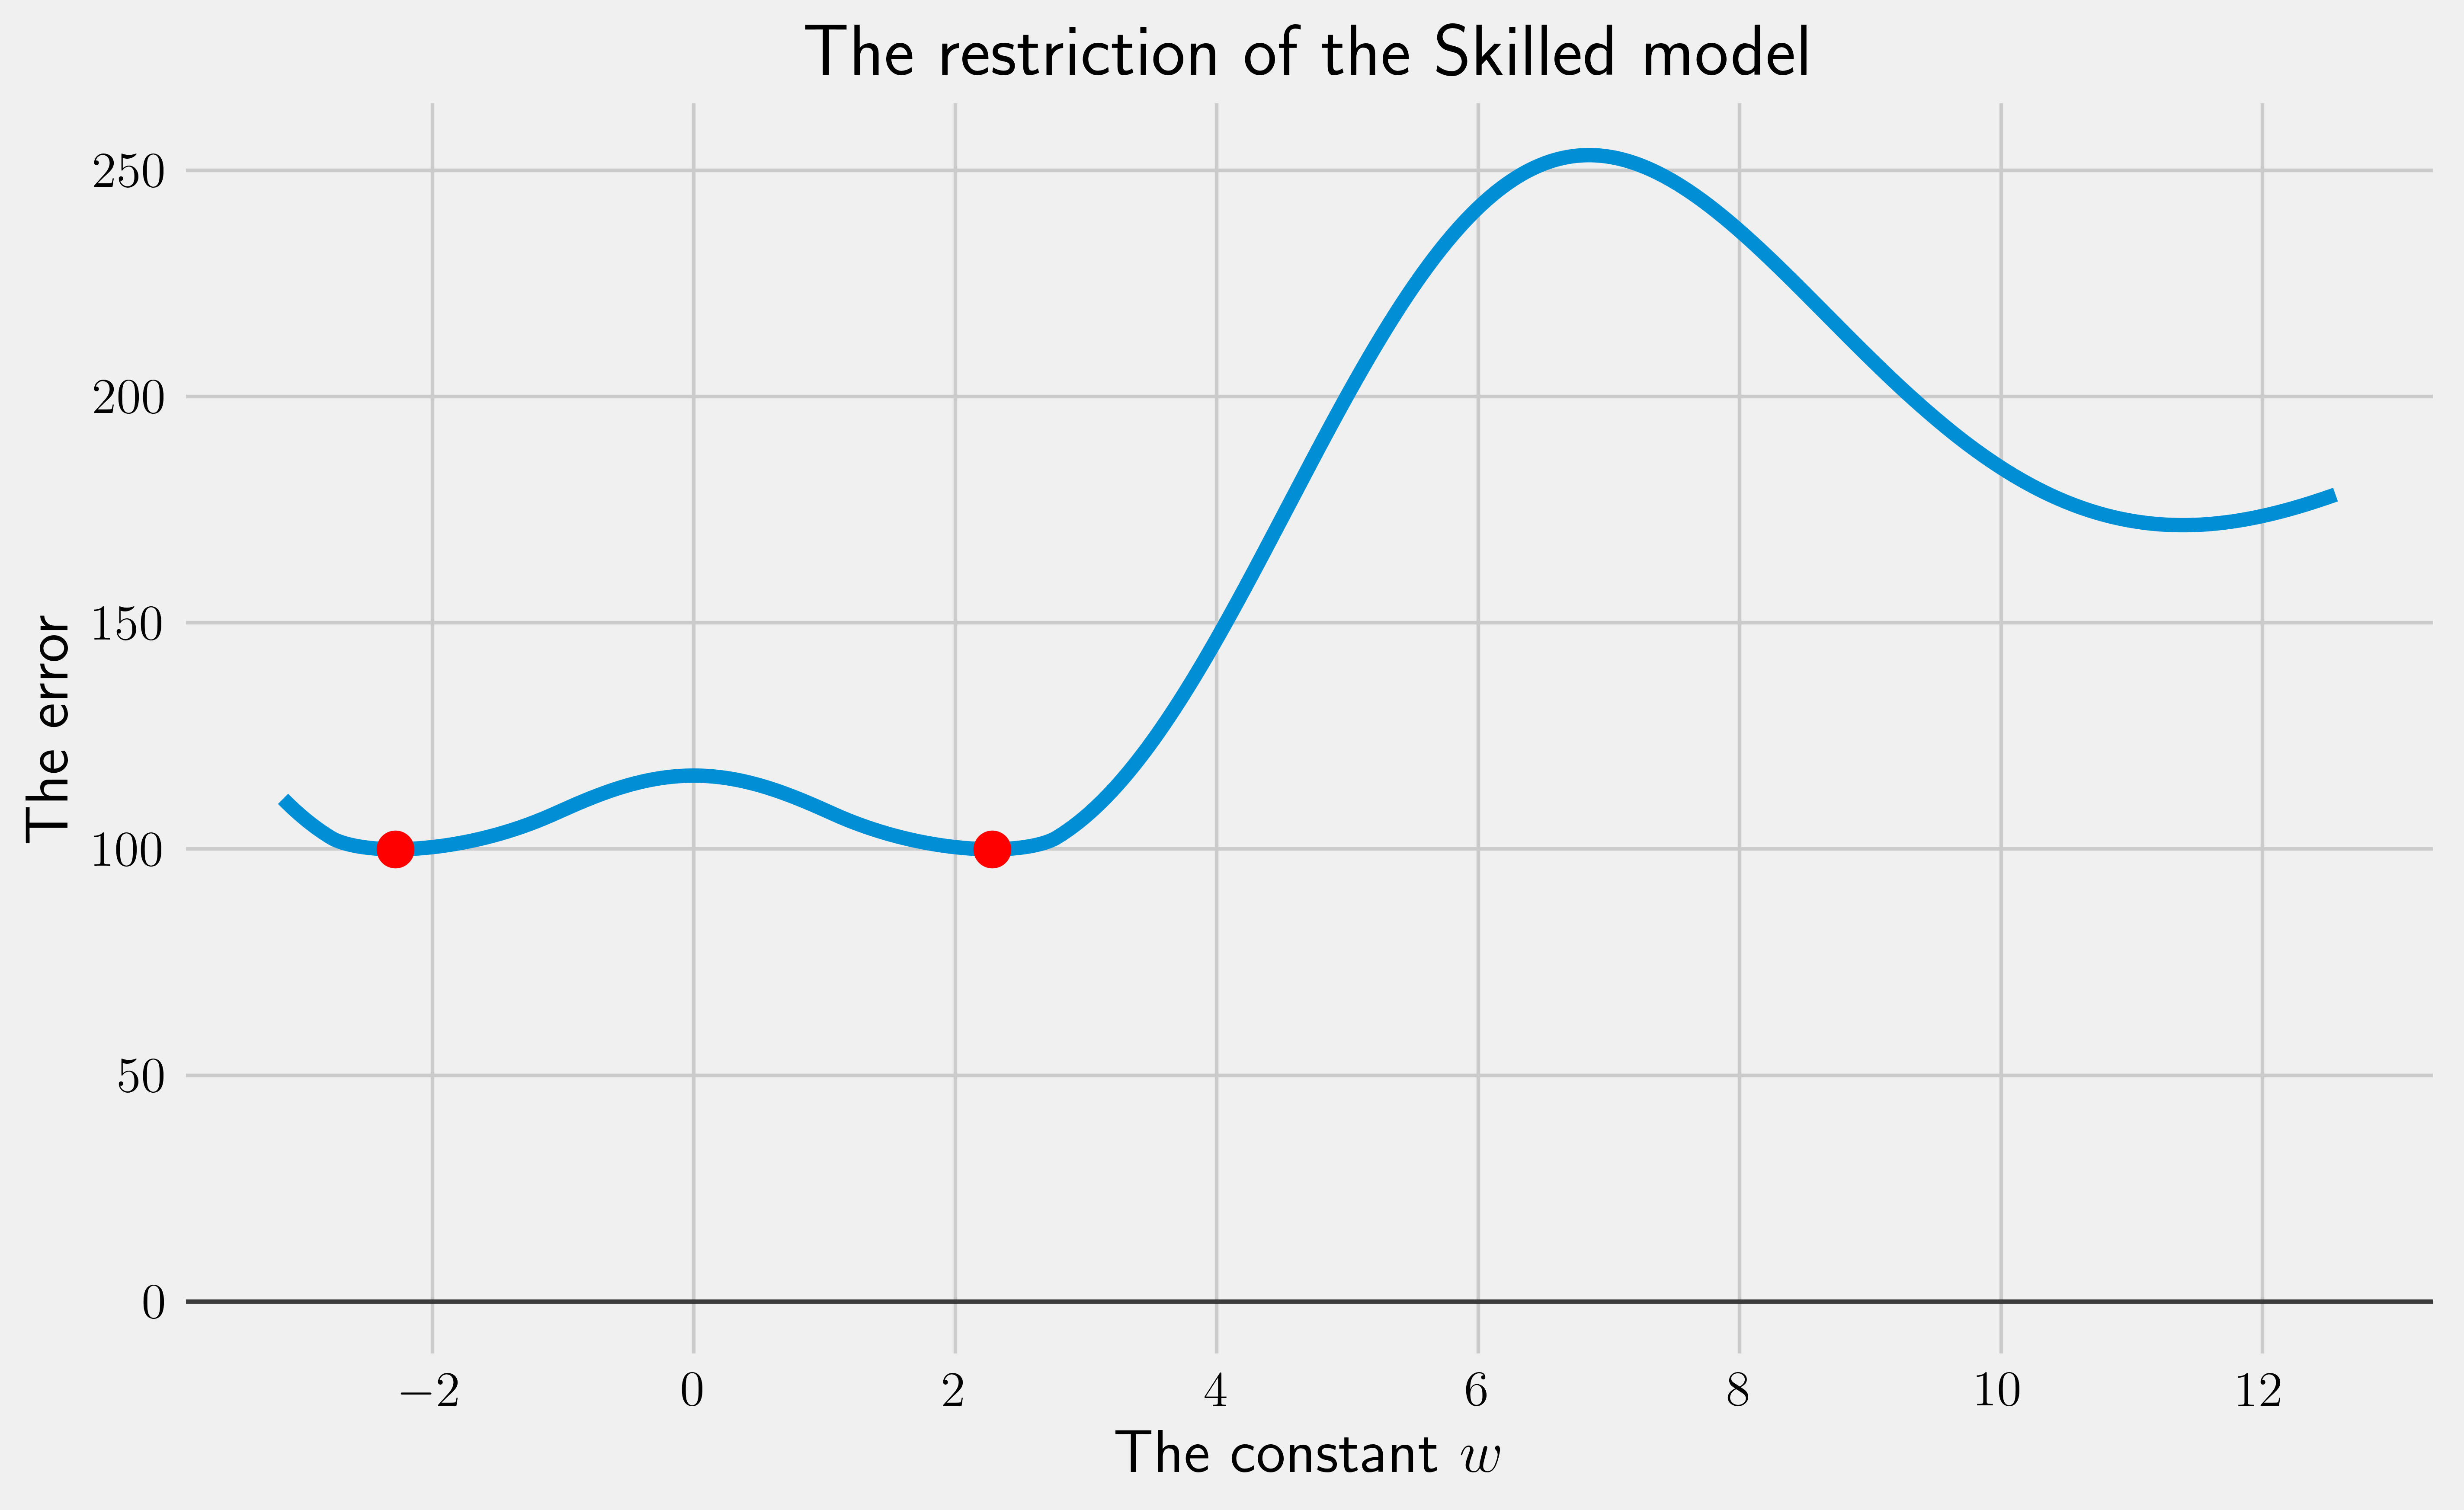
\includegraphics[width=0.85\textwidth]{assets/restriction_equation.png}
 \caption{}
 \label{fig:2error}
\end{figure}
% TODO: if needed, show the two red dots and choose the smallest one
Figure \ref{fig:2error} shows the graph of the error function in equation \ref{eq:2error}. While it may be possible to find the minimum of the error function using calculus, the steps are too complex and a numerical solution is taken instead shown by the red dot in the graph.

\begin{wrapfigure}{r}{0.50\textwidth}
    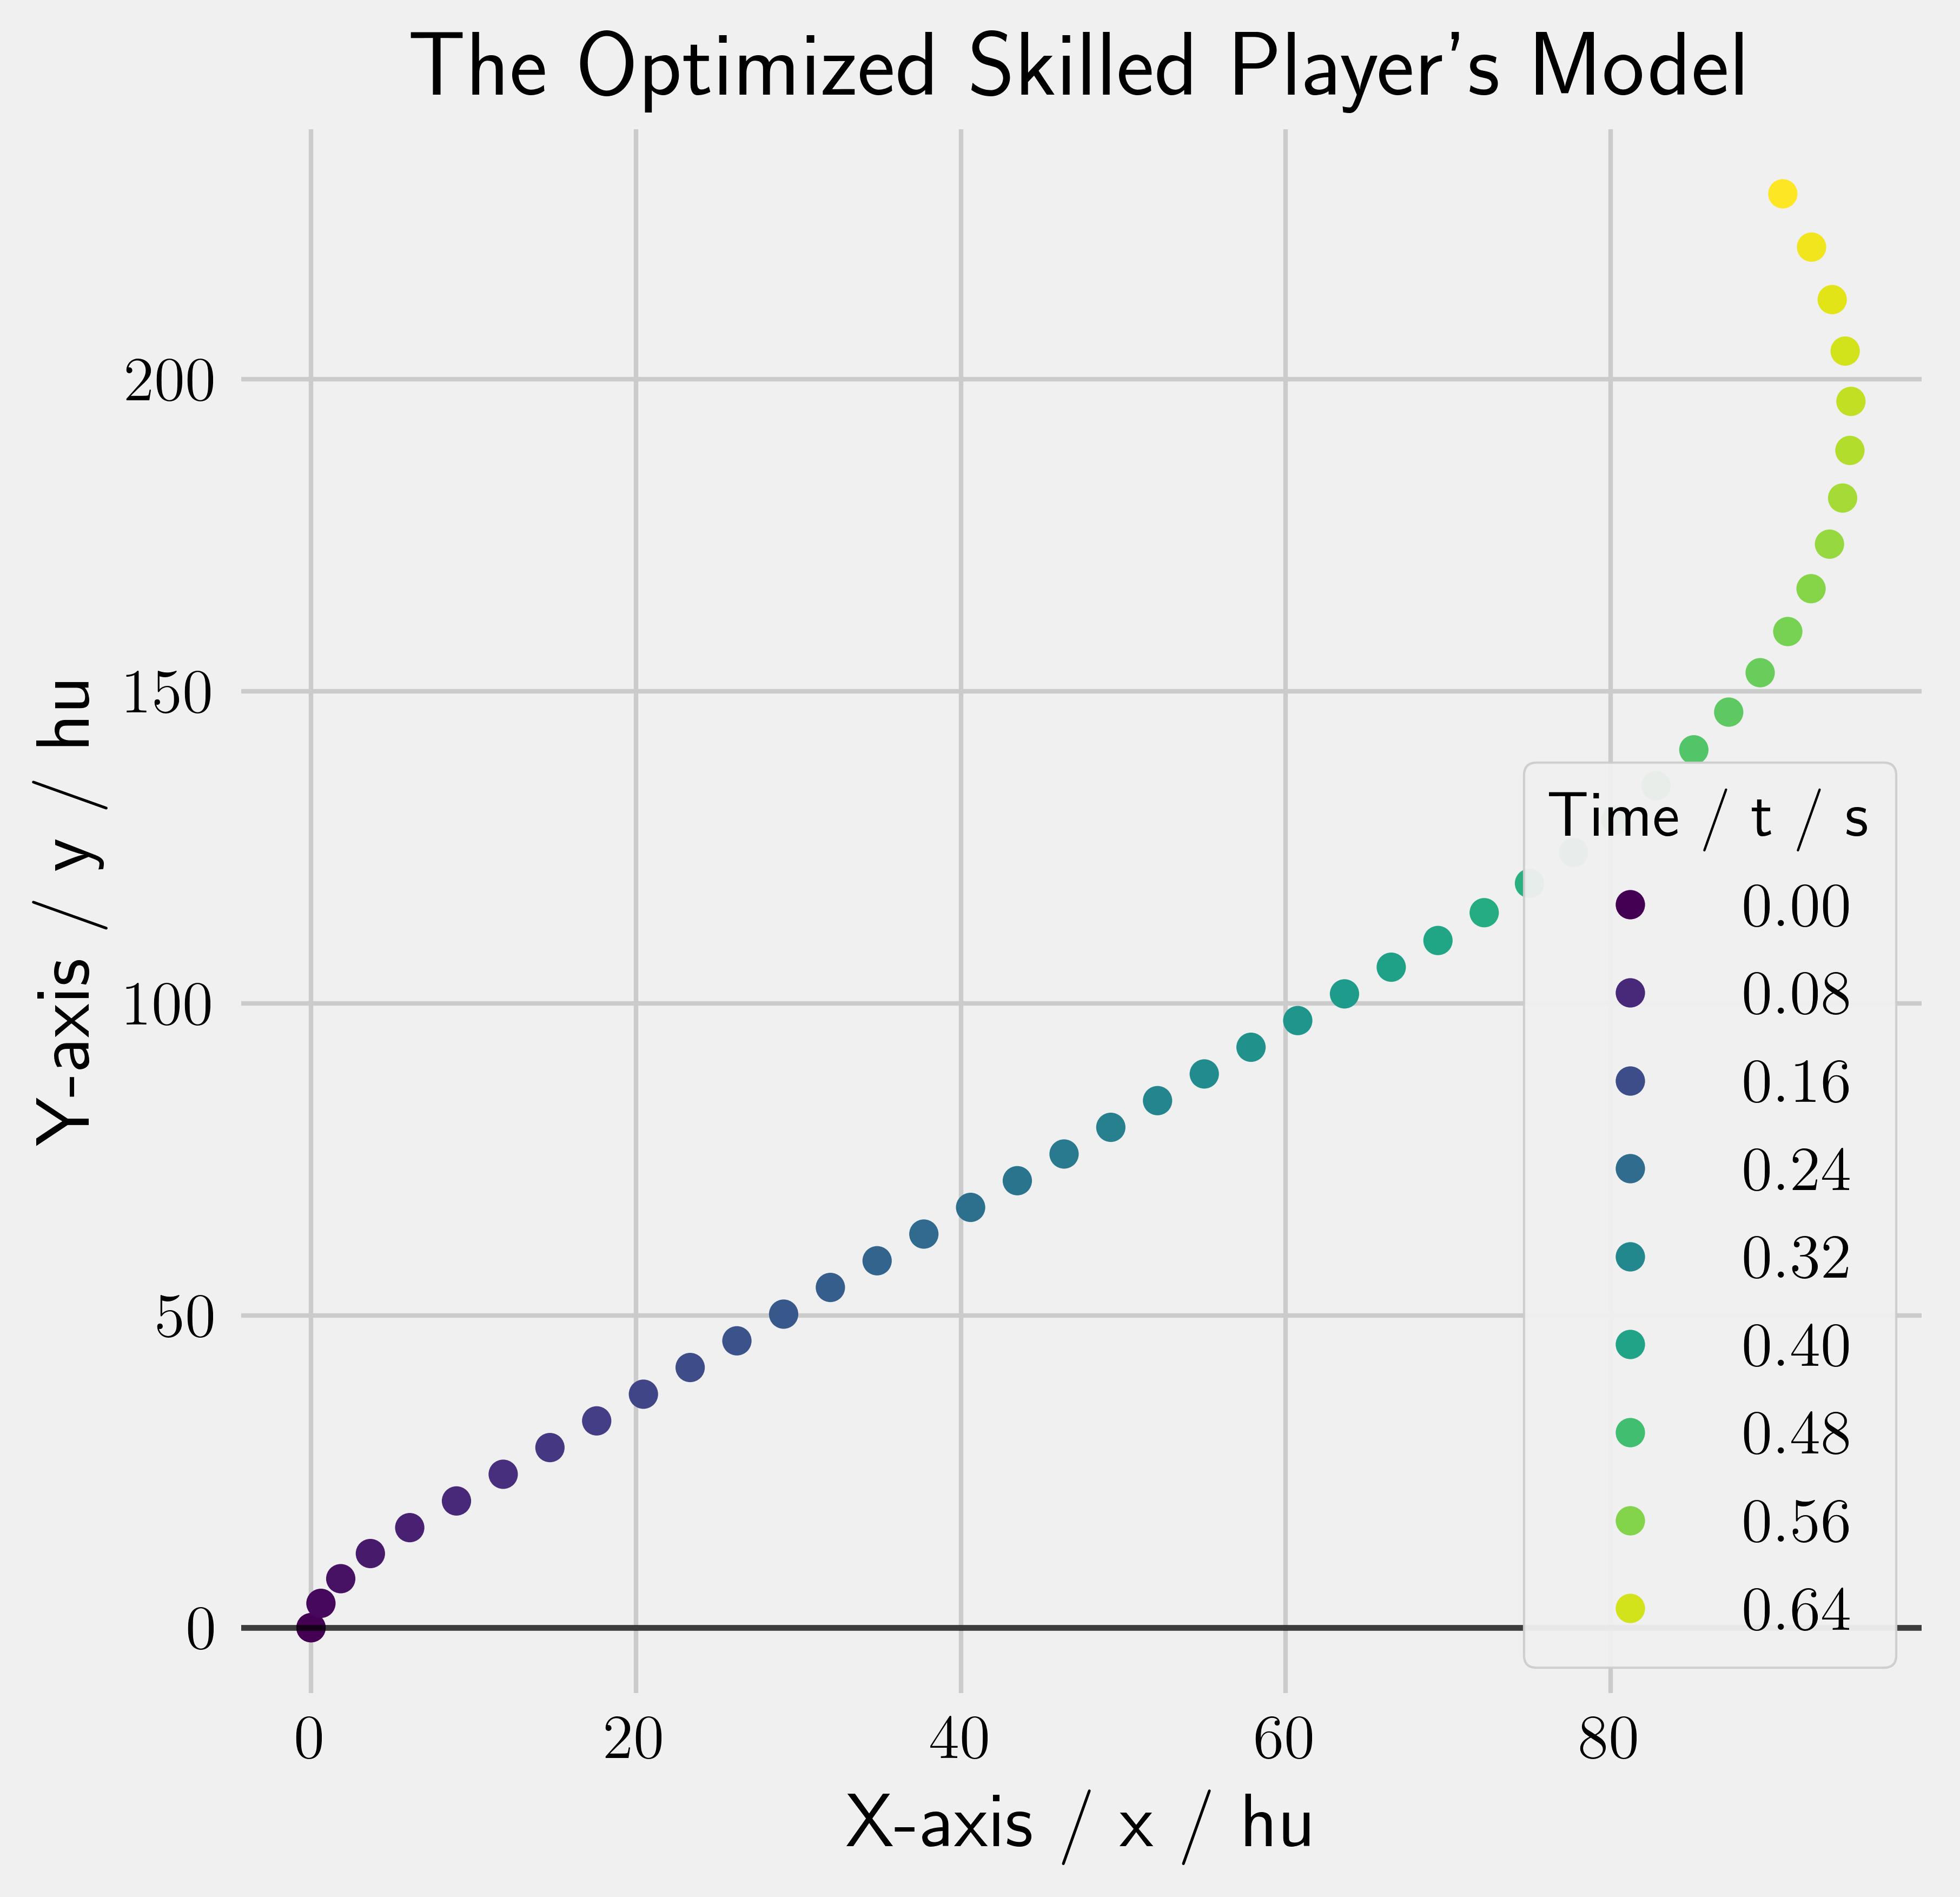
\includegraphics[width=0.47\textwidth,right]{assets/skilled_player.png}
    \caption{Skilled Player's Model}
    \label{fig:skilled_player}
\end{wrapfigure}

My program shows that the red dot is at coordinate
\[
    \tang{4.2884, 184.4228},
\]
meaning that the error function is the smallest with a constant of $w=4.2884$. I can therefore conclude that the skilled player's model is defined by
\[
    \td(t) = \tang{\sin(4.2884t), \cos(4.2884t)},
\]
indicating a relatively fast rate of turning at a period of $\frac{2\pi}{4.2884} = 1.4652\si{s}$.


Ideally, this optimized model corresponds to a displacement of $627.35$ using figure \ref{fig:skilled_displacement}. But I suspect the leftover ``$184.4228$'' errors to decrease the displacement by quite an amount. Figure \ref{fig:skilled_player} shows the actual path of the player when simulated in game; this is in combination with a correctly estimated lower displacement of $254.19$ units.
\begin{align*}
    \tp(t_f) &= \tang{88.3021, 238.3556}\\
    \tmag{\tp(t_f)} &\approx 254.19
\end{align*}

The skilled player's model does indeed produce a higher displacement ($254.19$) than the straight line model ($183.64$). Not only does this confirm the theory from these skilled people, but the large error of the even optimized model could indicate further possible optimizations when I look at the problem discretely.
